\section{Policy Modules}
\label{sec-policymodules}

Policy modules provide an interface through which applications can tune the
operation of the download manager.  As previously described, along with the
node-level utility assignment they make up the utility function responsible
for providing input to the download manager.  Lance requires that policy
modules be efficient in that they can process the stream of ADU summaries
received from the network in real time. In practice this is not difficult
to accomplish, as the rate of ADU summary reception is modest, and the base
station (typically a PC or laptop) is assumed to have adequate resources.
For example, a 100-node network with an ADU size of 60~sec would receive an
ADU summary every 600~msec. Typical policy modules take a small fraction of
this time to run. 

One of the main benefits of policy modules is that they permit significant
changes to the network's behavior {\em without requiring changes to the
node-level utility assignment}. Changing the latter would typically involve
reprogramming sensor nodes. Based on our experience at Reventador we were
wary of reprogramming the network unless absolutely necessary. Although
systems such as Deluge~\cite{deluge} permit over-the-air reprogramming, any
changes to the sensor node software could result in unexpected failures that
can be very difficult to debug without manual intervention.  On the other
hand, introducing new policy modules at the base station is relatively
straightforward, and can be quickly reversed without risking sensor node
failures. 

\subsection{Example Policy Modules}

Policy modules can be used to encapsulate a wide range of data collection
goals, and make it easy to customize Lance's behavior for specific
applications. While we provide a standard toolkit of general-purpose policy
modules, application developers are free to implement their own modules as
well.  By composing modules in a linear chain, it is easy to implement
various behaviors without requiring a general-purpose ``policy language.'' 

{\bf Priority thresholding:}
{\tt filter} is perhaps the simplest example of a policy module that filters
out ADUs with a utility below a given threshold $T$.  This type of filtering
can be used to force a drop of low-valued data. Conversely, the {\tt boost}
utility module sets the utility for an ADU above a given threshold to a
very high value, ensuring that it will be downloaded next. 

{\bf Priority adjustment and noise removal:} 
Policy modules can be used to remove the effects of noise or correct 
for node-level utility bias, for example, based on poor sensor 
calibration or differences in site response. Moreover, since each node 
computes the initial ADU utility based only on local sensor data, it may be 
necessary to normalize the ADU utilities in order to compare 
utilities across nodes. 

{\tt adjust} adds or subtracts a node-specific offset to each ADU utility
in order to correct for differences in sensor calibration. {\tt smooth}
applies a simple low-pass filter on the raw utility values to remove
spikes caused by spurious sensor noise.
Likewise, {\tt debias} is intended to remove
sensor-specific DC~bias in the utility values assigned by the node's
prioritization function. {\tt debias} computes the median utility
value for a given node over a given time window. It then subtracts
the median from each ADU utility before passing it along to the next
module in the chain. 

Likewise, when a sensor network contains
multiple sensors with varying sensitivity, it is natural to
prioritize data from more sensitive instruments. In cases where networks are
deployed to monitor fixed physical phenomena, it may be desirable to
prioritize data from nodes located close to the phenomena being
observed. The {\tt adjust} module can be used to scale
raw utilities based on a sensor's location, SNR, or other attributes.

{\bf Priority dilation:} 
Another useful policy is to dilate a high (or
low) utility value observed in one ADU across different ADUs sampled
at different times or different nodes. This can be used to achieve
greater spatial or temporal coverage of an interesting signal
observed at one or more nodes. The {\tt timespread} detects ADUs with
a utility above some threshold $T$, and 
assigns the same utility to those ADUs sampled just before and just
after.

Likewise, the {\tt spacespread} module groups ADUs from across multiple
nodes into time windows and assigns the maximum utility value to all
ADUs in that window.  Define a window $W(t,\delta)$ as the set of ADUs
such that $t-\delta \leq t_i \leq t+\delta$ where $t$ represents the
center of the window and $\delta$ the window size. {\tt spacespread}
determines the maximum ADU in the window $p^* = \arg_{i \in W} \max p_i$
and sets $p'_i = p^{*}$ for each ADU in $W$. 

\begin{figure}[t!]
\begin{center}
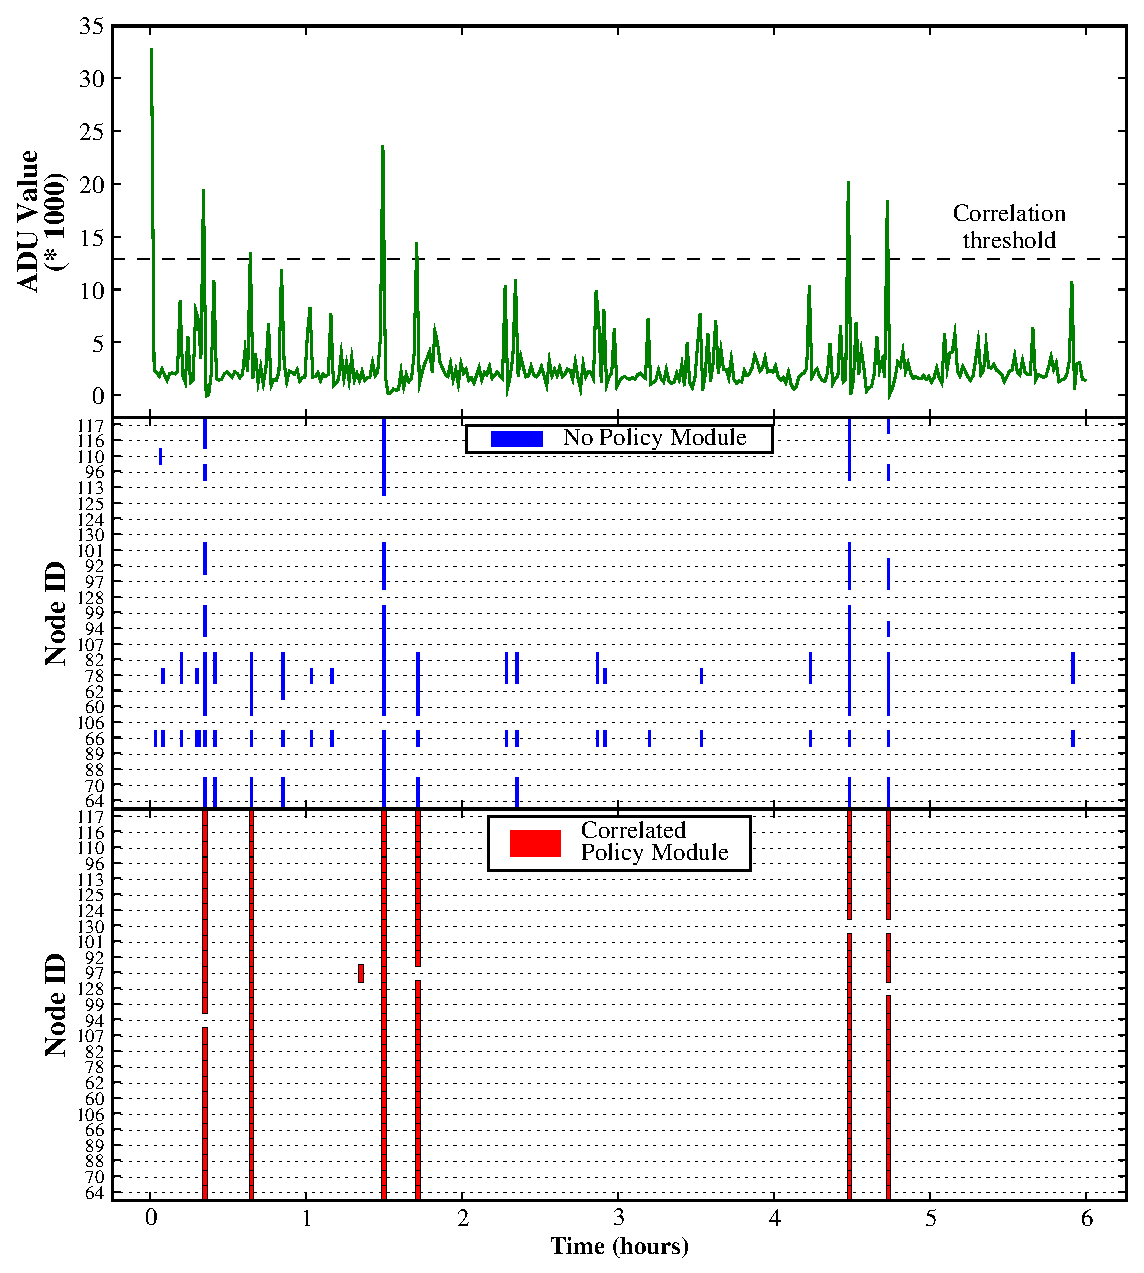
\includegraphics[width=1.0\hsize]{./figs/Sensys2008/2008-policy-module-usage.eps}
\end{center}
\caption{{\bf Usage of policy modules to affect download distribution.} 
Here we illustrate the use of policy modules. The graph compares the download
behavior of the system with and without a policy module chain which assigns
greater values to ADUs corresponding to correlated seismic activity.  The
graph is colored at a particular timestamp and node ID if we downloaded that
signal from that node. The top graph shows the ADU values over time, with the
threshold for the \texttt{filter} component of the policy module chain
indicated.}
\label{fig-policy-module-usage}
\end{figure}


{\bf Correlated event detection:}
The {\tt correlated} module is used to 
select for ADUs that appear to represent a correlated
event observed across the entire sensor network. 
{\tt correlated} counts the number of ADUs within a time window
$W(t,\delta)$ with a nonzero utility value.
If at least $k$ ADUs meet this criterion, we assume that there is 
a correlated stimulus, and the utility values for all ADUs in 
the set are passed through.  Otherwise, we filter out the ADUs in 
the window by setting $p'_i = 0$ for each ADU in $W$.

As an example of composing policy modules to implement an interesting
behavior, consider the chain \[
\mathit{filter}(T)\rightarrow\mathit{correlated}(k)\rightarrow\mathit{spacespread}
\] This policy filters incoming utilities, rejects time-correlated sets with
fewer than $k$ ADUs above the threshold, and assigns the max utility across
the set to all ADUs. This can be useful in systems that wish to perform
collection of time-correlated data, but avoid spurious high-utility data from
just a few nodes.  This policy is equivalent to the volcano earthquake
detector used in our previous work~\cite{volcano-osdi06}, expressed as a
simple policy module chain, and demonstrates, as mentioned in the previous
section, that our distributed event detector can be reimplemented as a Lance
utility function with both node- and network-level components.

\subsection{Evaluation and Use at Tungurahua}
\label{subsec-policymoduleuse}

We evaluated the usefulness of the policy module architecture through testbed
experiments, as well as during our field deployment in 2007.  For the testbed
experiment, we use a distribution of ADU data values based on a 6-hour
seismic trace collected at Reventador Volcano, Ecuador in
2005~\cite{volcano-osdi06}. The raw seismic data is divided into ADUs of 36
KB and ADU values $v_i$ are assigned by computing the ratio of two
EWMA~filters on the data, which assigns greater value to ADUs that contain
earthquakes. For each node in a 25 node topology, the ADU values from the
seismic trace are attenuated based on a hypothetical signal source and
assigned to each of the 25 nodes based on their location with respect to the
signal source. We then enable a policy module chain that assigns higher
priority to ADUs that correspond to correlated seismic activity across the
network.

Figure~\ref{fig-policy-module-usage} shows the result of this experiment
running on the MoteLab testbed. The upper portion of the figure shows the ADU
values over time; the middle portion, the set of ADUs downloaded by the
system with no policy modules in use; and the lower portion, the ADUs
downloaded with the policy module chain in use.  As the figure shows, the
policy modules cause the network to prefer correlated seismic events and
download an ADU from all nodes in the network when such an event is detected.
Gaps in the set of ADUs downloaded are due to download timeouts. In one case,
a single ADU is downloaded spuriously due to an incorrect value being
reported by that node to the base station. This use of policy modules shows
the drastic change in the system behavior that is affected without
programming the sensor nodes themselves.

Our deployment at Tungurahua Volcano allowed us to evaluate the ability to
change download policies at the base station without reprogramming nodes, one
of the significant advantages policy modules provide.  As described in
Sect.~\ref{subsubsec-rsamvewma}, the RSAM utility calculator initially
deployed at Tungurahua was sensitive to DC bias, which caused Lance to
continuously download signals from one or two nodes with large DC biases.

\begin{figure}[t!]
\begin{center}
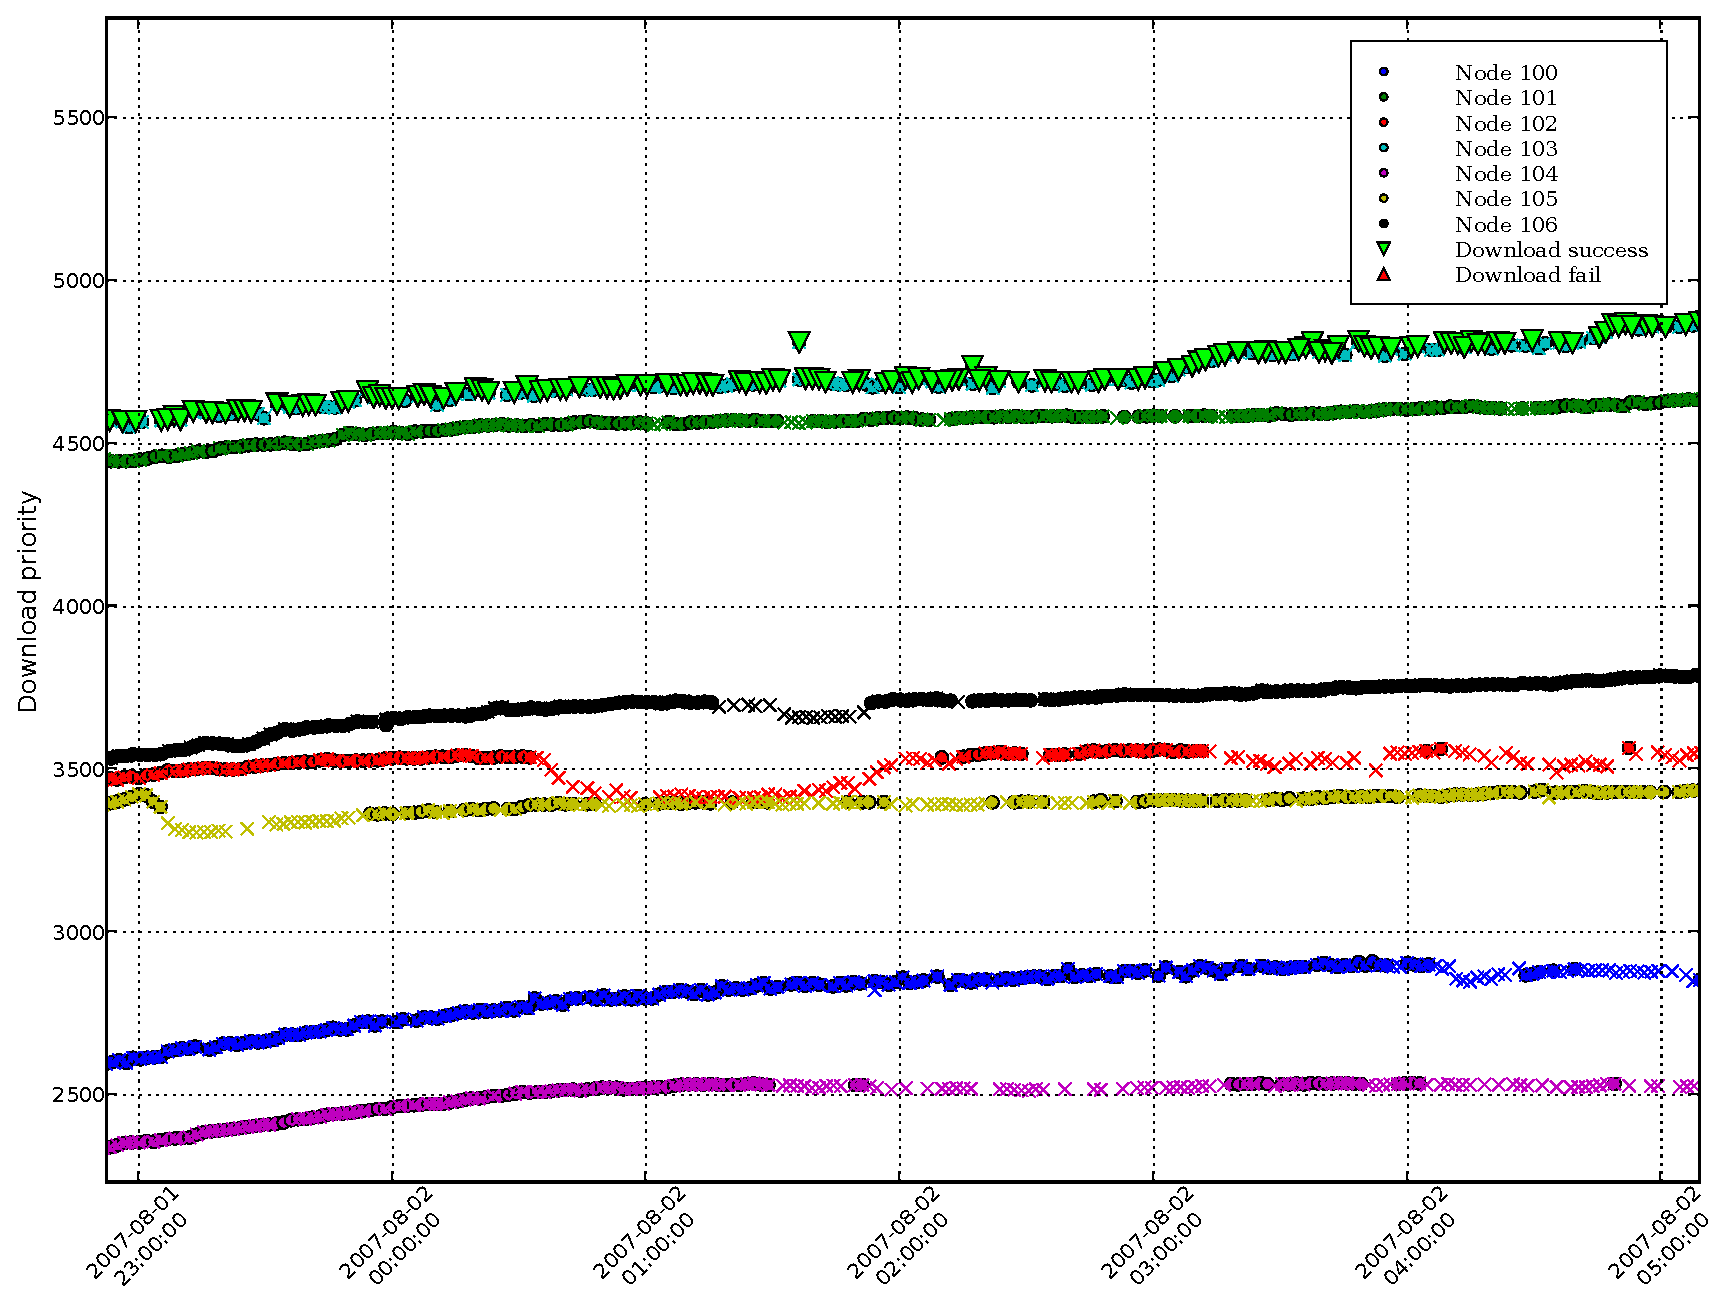
\includegraphics[width=0.7\hsize]{./figs/Sensys2008/2008-downloads-pre-median-filter.eps}\\
\textbf{(a)}\\
\includegraphics[width=0.7\hsize]{./figs/Sensys2008/2008-downloads-post-median-filter.eps}\\
\textbf{(b)}
\end{center}
\caption{{\bf Effect of DC bias on RSAM summarization function.}
Each point represents the ADU value received at the base station, and the
triangles indicate those ADUs that were downloaded by Lance. In \textbf{a},
because nodes' RSAM values are offset significantly from each other, Lance
prefers downloading from the node with the largest positive bias. However,
\textbf{b} shows what happens after applying a simple debiasing policy module
at the base station. This filter removes the DC bias causing Lance to
download from multiple nodes.}
\label{fig-downloads-median-filter}
\end{figure}

This problem was easily corrected, without any node software changes, by
introducing a policy module at the base station to process the raw RSAM
values received from each node and filter out the DC~bias. This was achieved
by computing the median RSAM value over each 30-minute window of raw RSAM
values on each node, and subtracting the median from the RSAM.
Figure~\ref{fig-downloads-median-filter} shows the result of the application
of the filter, with the debiasing effect clearly visible. The ability to
change and correct download behavior from the base station without modifying
sensor node code proved extremely useful in this case, particularly in that
it permitted the rapid iteration necessary to properly craft the appropriate
filter.
